

\documentclass[12pt]{article} 
\usepackage[utf8]{inputenc} % set input encoding (not needed with XeLaTeX)

\usepackage{geometry} \geometry{a4paper} 
\usepackage{graphicx} 
\usepackage{tikz}
\usetikzlibrary{shapes.geometric, arrows}
\tikzstyle{startstop} = [rectangle, rounded corners, minimum width=3cm, text width=3cm, minimum height=1cm,text centered, draw=black, fill=red!30]
\tikzstyle{io} = [trapezium, trapezium left angle=70, trapezium right angle=110,text width=3cm, minimum width=3cm, minimum height=1cm, text centered, draw=black, fill=blue!30]
\tikzstyle{process} = [rectangle, minimum width=3cm, minimum height=1cm, text centered, draw=black, text width=3cm, fill=orange!30]
\tikzstyle{decision} = [diamond, minimum width=3cm, minimum height=1cm,text width=3cm, text centered, draw=black, fill=green!30]
\tikzstyle{arrow} = [thick,->,>=stealth]



\begin{document}
\begin{center}
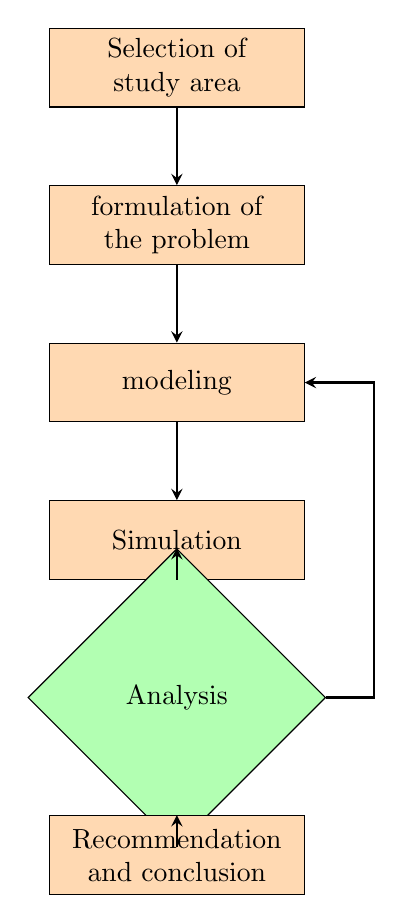
\begin{tikzpicture}[node distance=2cm]
	%\node (start) [startstop]{Start};	
	\node (p1) [process]{Selection of study area}; 
	\node (p2) [process, below of=p1]{formulation of the problem}; 
	\node (p3) [process, below of=p2]{modeling}; 
	\node (p4) [process, below of=p3]{Simulation}; 
	\node (d1) [decision, below of=p4]{Analysis}; 
	\node (p5) [process, below of=d1]{Recommendation and conclusion};
%\draw [arrow] (start) -- (p1);
\draw [arrow] (p1) -- (p2);
\draw [arrow] (p2) -- (p3);
\draw [arrow] (p3) -- (p4);
\draw [arrow] (p4) -- (d1);
\draw [arrow] (d1) -| + (2.5, 0) |- (p3);
\draw [arrow] (d1) -- (p5) ; 
\end{tikzpicture}
\end{center}
\end{document}
